\documentclass[10pt,parskip]{scrartcl}
%Options -- Point size:  10pt (default), 11pt, 12pt
%        -- Paper size:  letterpaper (default), a4paper, a5paper, b5paper
%                        legalpaper, executivepaper
%        -- Orientation  (portrait is the default)
%                        landscape
%        -- Print size:  oneside (default), twoside
%        -- Quality      final(default), draft
%        -- Title page   notitlepage, titlepage(default)
%        -- Columns      onecolumn(default), twocolumn
%        -- Equation numbering (equation numbers on the right is the default)
%                        leqno
%        -- Displayed equations (centered is the default)
%                        fleqn (equations start at the same distance from the right side)
%        -- Open bibliography style (closed is the default)
%                        openbib
% For instance the command
%           \documentclass[a4paper,12pt,leqno]{article}
% ensures that the paper size is a4, the fonts are typeset at the size 12p
% and the equation numbers are on the left side
%

\usepackage{listings}
\bibliographystyle{plain}
\usepackage[activate=normal]{pdfcprot}
\usepackage{url}
\usepackage{tabularx} %For word wrap
\usepackage{setspace}
\usepackage{ngerman}
%\usepackage[pdftex]{graphicx}
\usepackage{graphicx}

%
% PAGE LAYOUT
%
\setlength{\topmargin}{-1cm}
\setlength{\headheight}{1.5cm}
\setlength{\headsep}{0.3cm}
\setlength{\textheight}{23.5cm}
\setlength{\oddsidemargin}{0.5cm}
\setlength{\textwidth}{15cm}

\newcommand{\listingref}[1]{Listing \#\ref{#1}, on Page \pageref{#1}}
\setcounter{tocdepth}{2}
\setcounter{secnumdepth}{4}
% TOREAD: http://homepage.ruhr-uni-bochum.de/Georg.Verweyen/latexfuerword.html

% just some LaTeX parameters
%\hbadness=10
%\hfuzz=.01

% \input{}   ... insert file without new page
% \include{} ... insert file with new page

\lstset{tabsize=2}
\lstset{captionpos=b} %caption pos on bottom of the code
\lstset{breaklines=true}
\lstset{linewidth=\textwidth}
\lstset{basicstyle=\small\textit\ttfamily}


\begin{document}
\subject{Bakkalaureatsarbeit}
\author{Martin DOBIASCH \\MatNr:0828302\\Studium E-033-522 Informatikmanagement}
\title{NetLogo um Befehle f"ur Midi erweitern}
\date{2010-11-18}

% \frontmatter
% % (in)famous first page for the University of Vienna
% (in)famous first page for diploma thesis at the university of vienna

\begin{titlepage}
\begin{figure}[!b!t!h]
\hspace{8cm}
\includegraphics[width=7.2cm,height=2cm]{fig/uni_logo}
\end{figure}\par \vskip6em

\sffamily\mdseries{
\begin{center}
\textbf{\Huge BACHELORARBEIT}
\end{center} \vskip5.5em

\begin{center}
\textbf{\normalsize Titel der Bachelorarbeit }
\end{center}
\par \vskip1em
\begin{center}
\textbf{\huge Einsatz von Midi und NetLogo im Informatikunterricht}
\par \vskip1mm 
\textbf{\huge bzw. die Erweiterung von NetLogo um agentenbasierte Midi-Befehle}
\end{center} \par \vskip6em
\begin{center}
\textbf{\normalsize }
\end{center}
\par \vskip1em
\begin{center}
\textbf{\Large }
\end{center}
\par \vskip7em

\large
\begin{center}
\begin{tabbing}
Matrikel-Nummer: \hspace{1em} \= 0828302 \kill
Verfasser: \> Martin Dobiasch \\
Matrikel-Nummer: \> 0828302 \\
Studienrichtung: \> Informatikmanagement 522 \\
Betreuer: \> Ao. Univ.-Prof. Dr. Erich Neuwirth
\end{tabbing}
\end{center}

\par \vskip4em

%\begin{center}
\begin{tabbing}
Wien, am 18. 11. 2010 %TODO
\end{tabbing}
%\end{center}
}
\end{titlepage}


\begin{abstract}
Diese Arbeit beschreibt die Arbeit rund um die Erweiterung von NetLogo \cite{NetLogo} um 
Midi-Befehle f"ur die einzelnen Akteure (Turtles und Patches). 
%Diese Arbeit beschreibt das Projekt Midi f"ur NetLogo. 
Sie enthält Beispiele die im Informatik-Unterricht eingesetzt werden k"onnen
um Sch"ulerinnen und Sch"ulern einen technischen Zugang zu Problemen 
aufzuzeigen

\end{abstract}

\tableofcontents
\newpage

% \mainmatter %main part starts here

%\setcounter{chapter}{-1} % my first chapter starts with "0"

\section{Einleitung}
\subsection{Anreger \& Betreuer}
Auftraggeber und Betreuer dieser Arbeit war AO. Univ. Prof. Dr. Erich Neuwirth.
Ich m"ochte ihm hier an dieser Stelle bei ihm f"ur die ausgezeichnete Betreuung
und Zusammenarbeit bedanken.

\subsection{Ziel der Arbeit}
Die vorliegende Arbeit versteht sich als Arbeitsunterlage f"ur Lehrpersonen.
Nicht jedoch aber als Handout f"ur die Lernenden. Lehrende sollen durch dieses
Dokument einen Einblick in die verwendeten Tools bekommen und aufbereitete
Beispiele vorfinden, welche sie f"ur ihren Unterricht verwenden k"onnen.

Der Einsatz von Musik im Informatikunterricht mag auf den ersten Blick etwas
seltsam, wenn nicht sogar verst"orend wirken. Er bringt jedoch einen gro"sen
Vorteil mit sich: Fehler im Ansatz oder in der Ausarbeitung sind sofort
h"orbar. Ein falsch transponierter Dreiklang kann auch von einem musikalisch
nicht begabten Lernenden erkannt werden. Zu dem kann die Musik als m"achtiges
didaktisches Werkzeug gesehen werden, wenn es um die Vermittlung von parallelen
Verarbeitungsmodellen geht. Die Metapher eines Orchesters kann sehr gut heran
gezogen werden, da in ein Orchester aus mehreren MusikerInnen besteht. Diese
agieren von einander im wesentlichen unabh"angig, m"ussen jedoch bis zu einem
gewissen Grad von etwas bzw. jemand gesteuert werden: Dem Dirigenten, auf
englisch dem Condcutor. Auch die Metapher des Dirigenten/Conductor wird in 
meiner Arbeit stark zum Einsatz kommen. 

\emph{Wichtig f"ur einen Einsatz im Unterricht, ist der Hinweis, dass die
Lernenden Kopfh"orer mitbringen sollten.} Spielen mehrere ohne Kopfh"orer
ist ein Unterricht kaum mehr m"oglich und es herrscht Chaos. 

Beispiele daf"ur, was mit dem Toolkit m"oglich ist, finden sich im letzten 
Abschnitt. Es ist beispielsweise m"oglich, 2 Rettungsautos aus verschiedenen 
Richtungen fahren zu lassen und die Signalt"one der Autos akustisch zu lokalisieren.


\subsection{Verwendete Tools}
Im wesentlichen wird die NetLogo-Extension 'midi' verwendet. Die Midi-Extension
f"ur NetLogo enth"alt einige der F"ahigkeiten die das MidiCSD-Toolkit\cite{MidiCSD} f"ur 
OpenOffice bzw. Excel 
ebenfalls beherrscht. Der n"achste Abschnitt beschreibt die Notwendigkeit
der NetLogo-Erweiterung bzw. zeigt die Anleitung in 'Installation
der Erweiterung f"ur NetLogo' wie simpel sie zu installieren ist und
somit einfach im Unterricht eingesetzt werden kann. 
Es sei an dieser Stelle explizit auf MidiCSD hingewiesen. Gerade f"ur 
Experimente mit Musik eignet es sich hervorragend um im Informatik-Unterricht
angewendet zu werden. 

\subsection{Ausgangslage f"ur NetLogo}
\lstset{language=Logo}
Bisher st"orte die Tatsache, dass es nicht m"oglich war in NetLogo Midi-Kan"ale
direkt anzusprechen. In der Version 4.1.1 (aktuell zum Erstellungszeitpunkt des 
Projektes Juli, 2010) konnten lediglich die Befehle 
\lstinline|sound:play-drum drum velocity| und 
\lstinline|sound:play-note instrument keynumber velocity duration| verwendet
werden um Modelle mit T"onen zu versehen. %Das bedeutet aber gro"se 
%Einschr"ankungen. 
Als Konsequenz daraus konnte man den einzelnen Akteuren keine musikalischen Aktionen 
zuordnen. So ist es zum Beispiel nicht m"oglich f"ur das Beispiel 
''Rettungsauto'' (siehe \ref{Bsp:Rettungsauto}) den Dopplereffekt zu erzeugen,
geschweige denn "uberhaupt den Ton des Autos lauter werden zu lassen im Falle
des sich ann"ahernden Autos und wieder leiser werden zu lassen, im Fall des sich
entfernenden Autos. 

NetLogo hat eine (fast) unbeschr"ankte Anzahl an Akteuren, den Turtles. Bisher
war es aber nicht m"oglich Musik, oder einzelne T"one mit diesen zu verbinden.
Sieht man sich die Beispielsammlung der NetLogo-Distribution an, findet man im
Bereich Musik nur wenige Beispiele. Auch kann in diesen die volle Macht von
NetLogo nicht ausgenutzt werden. So wird z.B. im Beatbox Beispiel die Musik
von einer zentralen Prozedur aus angewandt. Alle 'Trommler' spielen jedoch
auf dem selben Midi-Kanal. Das w"are also so als w"urde doch nur ein Trommler spielen
und mehrere Percussioninstrumente zur gleichen Zeit bedienen.

Im vorigen Absatz wird erw"ahnt, dass nur auf einen Midi-Kanal zugegriffen wird.
Das ist wie schon eingangs erw"ahnt ein gro"ses Manko. Es ist also nicht
m"oglich Effekte nur f"ur einzelne Instrumente zu steuern. Beispiel: Der 
Trompeter soll leise spielen weil gerade die Fl"ote ein Solo hat (Funktioniert
im echten Leben leider auch nicht immer). 

\subsection{Installation der Erweiterung f"ur NetLogo}
Es gibt zwei Varianten um die Erweiterung zu installieren
\begin{itemize}
\item die Datei ''midi.jar'' in einen Unterordner ''midi'' neben das Model legen,
welches die Erweiterung verwenden m"ochte.
\item die Datei ''midi.jar'' in einen Ordner ''midi'' in das Verzeichnis ''extensions''
der NetLogo-Installation legen. 
\end{itemize}
Ebenso erfolgt die Installation f"ur als Applet im Internet hinterlegte Modelle.
Auch hier muss die ''midi.jar'' Datei ein einem ''midi'' Unterordner liegen.

\subsection{Gliederung der Arbeit}
Ich werde zuerst kurz beschreiben wie ich NetLogo um zus"atzliche Befehle erweitert
habe. Dann werde ich die Konzepte hinter der Erweiterung erl"autern und
Beispiele bringen wie die Befehle eingesetzt werden k"onnen. Diese Beispiele
sind schon so vorbereitet um in einem etwaigen Unterricht mit Sch"ulern eingesetzt
werden zu k"onnen. %Am Ende der Arbeit befinden sich die Listings der Erweiterung. 

Es werden einige Details hinter der Arbeit sehr ausf"uhrlich erl"autert. Dies 
wird gemacht um den Lesern bzw. Anwendern dieser Arbeit einen tieferen Einblick
in die Interna der Erweiterung zu geben. Ein tieferes Verst"andnis der Arbeit kann
einen verbesserten Einsatz im Unterricht erm"oglichen, da so jeder Lehrende 
individuell St"arken und Schw"achen f"ur den pers"onlichen Einsatz im Unterricht
ausmachen kann. Weiters tauchen in der Praxis der Informatik immer wieder Probleme
auf die nur durch ein detailliertes Wissen der verwendeten Mittel gel"ost werden
k"onnen. Auch r"ustet ein gutes Hintergrundwissen "uber die Erweiterung die
Lehrenden f"ur etwaige Fragen von interessierten Lernenden, welche zB die im
Unterricht erl"auterten Beispiele noch erweitern wollen oder bei der Erweiterung
auf Probleme gesto"sen sind. 

\subsection{Test der Erweiterung}
Da ein Teil meiner Arbeit war NetLogo\cite{NetLogo} Midi tauglich zu machen,
musste dies auch getestet werden. 
Die Arbeit wurde unter anderem mittels der weiter hinten in der Arbeit 
beschriebenen Beispiele
getestet. Es ist also gew"ahrleistet, dass diese Beispiele in der erl"auterten
Form funktionieren und keine Seiteneffekte hervorrufen. 
Getestet wurde sowohl auf Windows PCs so wie auf Apple Computern. 
Verwendet wurde die zum Zeitpunkt der Arbeit aktuelle NetLogo Version 4.1.1. 

Es wurden bei den Tests keine Unterschiede zwischen Windows und Mac OS entdeckt.

% \subsection{Einsatz in der Unterrichtspraxis}
% Die vorliegende Erweiterung kann direkt f"ur Unterrichtszwecke verwendet werden.
% Bei der Ausarbeitung der Beispiele weiter hinter hinten in der Arbeit wurde
% darauf geachtet sie m"oglichst gut aufzubereiten um sie direkt in Schulungen
% einsetzen zu k"onnen. Sie liegen liegen als fertig implementierte Modelle vor. 
% Die Modelle sind nicht direkt Teil meiner Arbeit. Sie wurden von Prof. Dr. Erich
% Neuwirth erdacht und ich habe sie in seiner Lehrveranstaltung ''Kernthemen der
% Fachdidaktik Informatik'' im Wintersemester 2009 kennen gelernt. 

\subsection{W"unschenswertes f"ur die NetLogo-Erweiterung}
Die Erweiterung wurde mit der Version 4.1.1 von NetLogo entwickelt. In geraumer
Zeit sollte die Version 4.1.2 fertig gestellt werden. Mit dieser Version kann
ein Problem meiner Erweiterung eventuell gel"ost werden und das hinzuf"ugen von
Befehlen zu Notenbl"attern direkt als Befehl m"oglich sein. Es seien hier einige
Aspekte aufgef"uhrt die von mir nicht in die Erweiterung aufgenommen wurden,
manch Lehrendem aber als fehlende Aspekte auffallen. Diese Liste erhebt aber keinen
Anspruch auf Vollst"andigkeit. Feedback von Lehrenden ist erw"unscht!

Die aktuelle Implementierung k"onnte noch in folgenden Punkten erweitert werden:
\begin{itemize}
\item \emph{Midi-Rendern} Es k"onnen zur zeit nur direkt Befehle ausgegeben 
werden. Eine m"ogliche Erweiterung ist, dass anstatt die Befehle auszugeben,
die akustische Ausgabe des Modells in ein Midi-File zu schreiben. 

\item \emph{Midi-Compiler} Wie sp"ater hinter in der Arbeit angemerkt wird, hat
die Implementierung Befehlsabarbeitung noch Potential zur Optimierung. Es k"onnte
angedacht werden, einzelne Bl"atter als Midi-Bl"atter zu deklarieren. Zu diesen
k"onnen dann nur Midi-Befehle hinzugef"ugt werden, welche dann direkt als javainterne
Midi-Commands kompiliert werden.

\item \emph{Protokollierung} Das Projekt k"onnte zus"atzlich um die Funktionalit"at
von Protokollausgaben der Befehle erweitert werden k"onnen. Anstatt von Midi-Noten
werden k"onnten dann normale Notennamen ausgegeben werden k"onnen. 

\end{itemize}


\section{Erweiterung}
\subsection{Grunds"atzliches}
Eine Extentsion f"ur NetLogo ist nichts anderes als ein Jar-Archiv. Die Erweiterung
muss in einem Unterverzeichnis des Models, welches die Erweiterung verwenden will,
oder in einem Unterverzeichnis des NetLogo-Programmes liegen. Jede Extension
ben"otigt einen ClassManager. Dieser teilt NetLogo mit welche Befehle die 
Erweiterung mit sich bringen wird. 
\lstset{language=Java} Jeder dieser Befehle ist von \lstinline|org.nlogo.api.Primitive|
abgeleitet. Die Erweiterung muss zus"atzlich ein Manifest mit den folgenden 
Befehlen enthalten (am Beispiel meiner Erweiterung):
\begin{verbatim}
Manifest-Version: 1.0
Extension-Name: midi
Class-Manager: at.univie.csd.MidiManager
NetLogo-Extension-API-Version: 4.1
\end{verbatim}

\subsection{Unterlagen}
F"ur die Erstellung der Erweiterung wurden im wesentlich folgende Quellen 
zu Theorie zu Midi zur Rate gezogen: \cite{midi-inst}, \cite{midi-java} und
\cite{midi-javafaq} verwendet. 


\subsection{Struktur}
\begin{figure}[hbt]
	\centering
		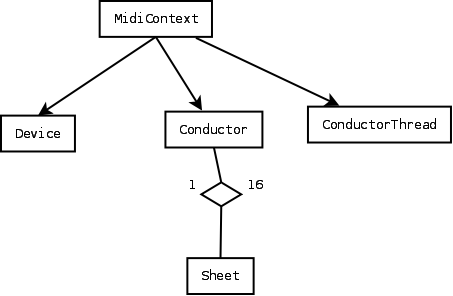
\includegraphics[scale=0.5]{fig/struktur.png}
	\caption{Struktur}
	\label{fig:struktur}
\end{figure}
Die Erweiterung besitzt eine relativ einfache Struktur. Beim laden der Erweiterung
wird eine \lstinline|MidiContext| Instanz erzeugt. Um eine Synchronisation der
Zugriffe auf die Objekte zu erm"oglichen habe ich in Anlehnung an \cite{fh-wedel} 
einfache Semaphore implementiert. Anstatt von Integerz"ahlern habe ich einfach
boolesche Variablen verwendet. Bei den Tests hat dies zu keinen Problemen gef"uhrt.
Zu finden sind die Semaphore in der Klasse MidiContext in der Datei 
''MidiContext.java''. 

Die Implementierung als Semaphor mit Z"ahler w"urde wie folgt aussehen:
\begin{lstlisting}[language=Java,basicstyle=\small]
	...
	private int m_free = 1;
	...
	public synchronized MidiDevice getDevice()
	{
		while( m_free <= 0 )
		{
			try
			{
				wait();
			}
			catch(InterruptedException e)
			{
			}
		}
		m_free--;
	}
	...
	public synchronized void releaseDevice()
	{
		m_free++;
		notify();
	}
\end{lstlisting}
Analog die Impelentierung f"ur den Conductor-Semaphor. 
\subsubsection{MidiContext}
Der MidiContext soll sich um die Synchronisation der Threads k"ummern. Da nur
ein Device zum abspielen der MidiBefehle ge"offnet wird muss der Zugriff 
synchronisiert werden. Um einen Befehl schreiben zu k"onnen muss zuerst der
Zugriff reserviert werden. Dies geschieht "uber den Befehl
\lstinline|MidiManager.getMidiContext().getDevice();|. Nat"urlich muss auch noch
"uberpr"uft werden ob das Device auch offen ist. Um das Device wieder f"ur andere
Threads wieder frei zu geben muss der Befehl
\lstinline|MidiManager.getMidiContext().releaseDevice();| verwendet werden. 

\subsubsection{Conductor}
Weiters beinhaltet der MidiContext eine Instanz des Conductors. Diese Klasse 
soll helfen einen virtuellen Dirigenten zu erstellen. Dazu hat die Klasse 
bis zu 16 Notenbl"atter. Die Anzahl ist Aufgrund der Midi-Spezifikation von
16 Kan"alen festgesetzt worden. Auch hier muss wieder um die Synchronit"at 
zugew"ahrleisten mit den Befehlen \lstinline|MidiManager.getMidiContext().getConductor();|
und \lstinline|MidiManager.getMidiContext().releaseConductor();| gearbeitet 
werden. 

\subsubsection{Sheet}
Die Klasse Sheet hilft bei der Verwaltung von Kommandos, die timecode gesteuert
ausgef"uhrt werden sollen. Sheet ist das Pendant zu Streams in MidiCSD \cite{MidiCSD}
Jedes Notenblatt verf"ugt "uber eine Liste von Kommandos. Zu Begin der Arbeit
war die Anzahl dieser Commandos auf die des MidiCSD-Toolkits beschr"ankt und 
jeder dieser Befehle wurde intern zu den entsprechenden Midi-Befehlen kompiliert.
Dies wurde jedoch in R"ucksprache und auf Wunsch des Betreuers so ge"andert, 
dass nun jedes beliebige Kommando hinzugef"ugt werden kann. W"ahrend des
Programmablaufes wird also das Kommando nur gespeichert und dann NetLogo zur
Ausf"uhrung "ubergeben. Dies f"uhrt zu kleinen Laufzeiteinbusen, erh"oht jedoch
aber die Flexibilit"at und erweitert die M"oglichkeiten f"ur den Einsatz der 
Erweiterung. So ist es zum Beispiel m"oglich den virtuellen Musikern nicht nur
Noten sondern auch Bewegungen beizubringen. 
Der ''alte'' Code wurde als Kommentar im Source-Code hinterlassen. 

\subsubsection{ConductorThread}
Damit der Dirigent im Hintergrund die Notenbl"atter abarbeiten kann, wurde der
CondutorThread erstellt. Dieser, wenn gestartet, arbeitet St"uck f"ur St"uck
die Notenbl"atter ab. Dies macht er, in dem er sich in jedem Schritt einen
Zugriff auf den Conductor reserviert um sich die anstehenden Kommandos zu besorgen.
Diese werden dann sequentiell ausgef"uhrt. Danach legt sich der ConductorThread
f"ur 100ms schlafen um den anderen Threads nicht im Weg zu stehen. 

\subsection{Neue Befehle}
Um einfach neue Midi-Befehle implementieren zu k"onnen habe ich eine Klasse
\lstinline|MidiCommand| geschrieben. Diese besitzt im wesentlichen zwei 
Methoden: \lstinline|preAction| und \lstinline|postAction|. Jeder neue Midi-Befehl,
wenn von dieser Klasse abgeleitet, kann sich \lstinline|preAction| Zugriff auf
das Midi-Device holen und diesen dann wieder mit \lstinline|postAction| freigeben.
So kann sicher gestellt werden, dass durch neue Befehle kein Wirrwarr von offenen
Devices entsteht. Weiters erh"oht diese Vorgangsweise die Modularit"at. Soll zum
Beispiel etwas an der Art wie das Device ge"offnet wird ge"andert werden, muss
dies nur an einer Stelle angepasst werden. 



\section{Der Dirigent in Midi-NetLogo}
Ein weiterer Punkt den ich in die Aufgabenstellung inkludiert habe, war die
M"oglichkeit Sequenzen zu definieren, welche dann unabh"angig abspielbar sein 
sollen. Dieser Punkt wurde dann erweitert, dass es m"oglich sein soll, alle
in NetLogo verf"ugbaren Befehle in so eine Sequenz zu packen. 

Das kann nun daf"ur verwendet werden um im Informatik-Unterricht Threads zu
vermitteln. Ein Thread ist damit nichts anderes als ein Sheet. 

\subsection{Konzept}
Wie der Name schon andeutet, ist dieser Aspekt mit der Metapher eines Orchesters
gel"ost worden. Ein Dirigent hat die Kontrolle "uber mehrere Musiker die 
Aktionen ausf"uhren sollen. Er bestimmt wann das Orchester zu spielen beginnt
und wann es wieder aufh"ort. Weiters kann er nat"urlich auch wieder von Vorne
beginnen lassen.

Jedes Programm braucht auch Mechanismen zur Steuerung und Synchronisation 
seiner Threads. Der Dirigent "ubernimmt diese Aufgabe und erm"oglicht so eine
vereinfachte Form der Vermittlung von Thread-Synchronisation. 

\subsection{Technische Realisierung}
Wie schon im Konzept erw"ahnt wird NetLogo durch die Midi-Extension eine Zentrale Instanz 'Conductor'
beigebracht. Diese verf"ugt "uber die folgenden F"ahigkeiten: \begin{itemize}
\item Alle Notenbl"atter l"oschen
\item Zu einem Notenblatt etwas hinzuf"ugen
\item Zu einem Notenblatt einen mit Timecode versehenen Befehl hinzuf"ugen
\item Alles auf Anfang setzen
\item Dirigieren
\item Endlos spielen lassen, normal spielen lassen
\end{itemize}

\subsubsection{Sheets - Kan"ale}\label{sec:sheet-channel}
Der Dirigent h"alt eine fixe Anzahl von 16 Sheets. Die Zahl ist so festgelegt,
da Midi 16 Kan"ale besitzt. Die Midi-Kan"ale besitzen die Nummern 1 - 16, die
Sheets jedoch die Indizes/Nummern 0 - 15. "Uber eine Variable f"ur Agents kann
eine Zuordnung von Agenten zu einem Kanal gemacht werden. 
\begin{lstlisting}[language=Logo]
turtles-own [channel]
...
to init
  den Turtles channels zu ordnen
end

...

to some.procedure
	ask turtles[
		midi:instrument channel 60
	]
end
\end{lstlisting}
Eine sehr einfach Variante den Turtles Kan"ale zuzuornen ist:
\begin{lstlisting}[language=Logo]
ask turtles[
	set channel who + 1
]
\end{lstlisting}

\subsubsection{Events}
Die zentrale Aufgabe der Sheets ist es Befehle in chronologischer Reihenfolge
auszuf"uhren. Es gibt zwei Befehle um einem Notenblatt Befehle hinzu zuf"ugen:
\begin{itemize}
\item conductor.add.to.sheet
\item conductor.add.to.sheet.list
\end{itemize}
Beide Befehle machen im wesentlichen das Gleiche, jedoch werden dem Zweiten
eine Liste von mit einem Timecode versehenen Befehlen "ubergeben, ersterer f"ugt
einen einzelnen Befehl versehen mit einem Timecode zu einem Notenblatt hinzu. 
Eine genauere Beschreibung ist im Kapitel "uber die Befehle zu finden. 




\section{Befehle der NetLogo-Extension}
Alle Befehle beginnen mit einem vorangestellten \lstinline|midi:|. 
Ich m"ochte hier kurz die Befehle beschreiben um der Lehrperson einen tieferen 
Einblick zu gew"ahren und damit diese den Lernenden bei etwaigen Problemen kompetent
helfen k"onnen. 

Die Dokumentation der Befehle erfolgt immer in der Form \lstinline|Befehl Parameter|
was dann in einem NetLogo-Programm als \lstinline|midi:Befehl Parameter| geschrieben
wird. Die Befehlsnamen sind nicht(!) casesensitive. 
\subsection{Midi-Befehle}
\subsubsection{Standard Befehle}
Auf eine Dokumentation der Standard-Midi-Befehle m"ochte ich hier verzichten. Es sei
auf das Studium einschl"agiger Fachliteratur verwiesen. 
Folgende Befehle sind in der Erweiterung verf"ugbar: 
noteon,
noteoff,
instrument (F"ur eine Liste an Instrumenten siehe \cite{midi-inst}),
pitch.bend,
controller,
key.pressure,
channel.pressure,
volume,
expression,
modulation,
pan,
sustain,
reverb,
chorus,
portamento.time,
portamento,
portamento.from,
rpn,
nrpn,
reset.controllers,
all.notes.off,
pitch.sens channel,
mastertune.coarse,
mastertune.fine,
panic
% \subsubsection{Standard Befehle}
% \begin{itemize}
% \item \lstinline|noteon channel note volume|
% \item \lstinline|noteoff channel note|
% \item \lstinline|instrument channel instrument| (F"ur eine Liste an Instrumenten
% siehe \cite{midi-inst}
% \item \lstinline|pitch.bend channel bend|
% \item \lstinline|controller channel controller parameter|
% \item \lstinline|key.pressure channel note pressure|
% \item \lstinline|channel.pressure channel pressure|
% \item \lstinline|volume channel volume|
% \item \lstinline|expression channel expression|
% \item \lstinline|modulation channel modulation|
% \item \lstinline|pan channel pan|
% \item \lstinline|sustain channel value|
% \item \lstinline|reverb channel note volume duration|
% \item \lstinline|chorus channel duration|
% \item \lstinline|portamento.time channel time|
% \item \lstinline|portamento channel onoff|
% \item \lstinline|portamento.from channel note|
% \item \lstinline|rpn channel lorpn hirpn lodata hidata|
% \item \lstinline|nrpn channel lorpn hirpn lodata hidata|
% \item \lstinline|reset.controllers channel|
% \item \lstinline|all.notes.off channel|
% \item \lstinline|pitch.sens channel semitones|
% \item \lstinline|mastertune.coarse channel hidata|
% \item \lstinline|mastertune.fine channel cents|
% \item \lstinline|panic|
% \end{itemize}
\subsubsection{Der Note Befehle}
\lstinline|note channel note volume duration| \label{note-warning}


\begin{emph}Achtung: Dieser
Befehl ist ein Blocking-Call. Er spielt eine Noten in der Dauer von 
\lstinline|duration| (in ms angegeben ab). Erst dann wird das Programm fortgesetzt.
Er setzt zuerst die Note und legt den Thread dann schlafen, nach Abwarten des
Notenwertes l"oscht er die Note vom entsprechenden Midi-Kanal. Dieses Verhalten
kann zu Problemen f"uhren wenn sie in Programmen in Kombination mit den 
Conductor-Utilities verwendet werden. \end{emph}
\subsection{Befehle f"ur Turtles/Agenten}
\lstinline|updatepostion channel| 

Dieser Befehl setzt eine eine Position im akustischen Raum f"ur die aktuelle
Turtle, kann also nur in einem Turtle-Context angewandt werden. Die Position
wird f"ur die Turtle die den Befehl aufruft errechnet und dann als virtuelle
Position auf den "ubergebenen Channel gelegt (siehe auch \ref{sec:sheet-channel}. 
Ver"andert werden die Parameter Pan und Expression. Ausgangspunkt f"ur die
Berechnung ist der Koordinaten-Ursprung des NetLogo-Models. Als maximaler Wert
f"ur die Skalierung wird auch jeweils der maximale Wert des Koordinatensystems
verwendet wird. Das hei"st wenn das Model zB. auf der positiven X-Achse mehr Werte
zul"asst als auf der negativen. Ist die Abstufung auf der positiven Seite feiner.

\subsection{Befehle f"ur den Condcutor}
\subsubsection{clear.sheets}
Syntax: \lstinline|conductor.clear.sheets|

L"oscht alle dem Conductor bekannten Notenbl"atter.
\subsubsection{add.to.sheet}
Syntax: \lstinline|conductor.add.to.sheet sheet time.distance command|

Dieser Befehl f"ugt dem angegebenen Notenblatt am Ende ein Kommando hinzu. Das
Kommando wird nach Ablauf der durch \lstinline|time.distance| angegebenen Zeit
(in ms) ausgef"uhrt. Zus"atzlich ist das der Zeitpunkt von welchem aus der 
Zeitpunkt f"ur ein m"ogliches nachfolgendes Kommando berechnet wird. Beispiel:
\begin{lstlisting}[language=Logo]
midi:conductor.clear.sheets
midi:conductor.add.to.sheet 1 10 "midi:noteon 2 60 1"
midi:conductor.add.to.sheet 1 2000 "midi:noteoff 2 60"
midi:conductor.start
\end{lstlisting}
Nach Ablauf von zehn Milisekunden wird vom Notenblatt Eins auf dem Midi-Kanal
Zwei die Note mit dem Wert 60 gespielt. Nach zwei Sekunden, also nach insgesamt
2010 Milisekunden verstummt die Note wieder. 

\subsubsection{add.to.sheet.list}
Syntax: \lstinline|conductor.add.to.sheet.list sheet command.list|

Dieses Kommando f"ugt dem angegebenen Notenblatt am Ende die Kommandos aus der 
Liste ein. Die Kommando-Liste hat eine einfache Syntax: \lstinline|[time.code command]|
Die Time-Codes funktionieren analog zu denen des \lstinline|add.to.sheet| Befehls.
Das Kommando muss aber als String angegeben werden! Das kommt daher, dass NetLogo
zum Entwicklungszeitpunkt (Juli-Oktober 2010) nicht ausreichend mit dem Syntax-Typ
''Command'' umgehen konnte. Die Befehle sollten also getestet werden bevor sie
auf die Notenbl"atter geschrieben werden. Der Vorteil dieses Befehls ist, dass
er, mit geringen Modifikationen, die Ausgabe des ''to Logo'' des MidiCSD-Toolkits \cite{MidiCSD}
f"ur Office Dr. Erich Neuwirth verwendet kann. Das untenstehende Beispiel demonstriert,
wie der Befehl eingesetzt werden kann. 
\begin{lstlisting}[language=Logo]
to trommler
  clear-all
  midi:conductor.clear.sheets
 
  midi:conductor.add.to.sheet.list 1 [
		[0 "midi:note 10 45 1 200"]
		[200 "midi:note 10 45 0.7 200"]
		[200 "midi:note 10 45 0.7 200"]
		[200 "midi:note 10 45 0.7 200"]
		[200 "midi:note 10 45 1 200"]
  ]
  midi:conductor.add.to.sheet.list 2 [
		[200 "midi:pan 10 -0.75"]
		[200 "midi:pan 10 -0.5"]
		[200 "midi:pan 10 -0.25"]
		[200 "midi:pan 10 0"]
  ]
  
  midi:conductor.add.to.sheet.list 3 [
		[5 "midi:expression 10 0.75"]
		[200 "midi:expression 10 0.69"]
		[200 "midi:expression 10 0.63"]
		[200 "midi:expression 10 0.56"]
		[200 "midi:expression 10 0.5"]
  ]
  
  midi:conductor.setplaymode.endless

  midi:conductor.start
end
\end{lstlisting}

\subsubsection{restart}
Syntax: \lstinline|conductor.restart|

Die Position auf den Notenbl"attern wird wieder auf Null gesetzt. Alle Notenbl"atter
werden also wieder von Vorne abgearbeitet. 
\subsubsection{conduct}
Syntax: \lstinline|conductor.conduct|

Der Dirigent wird angewiesen die aktuell anfallenden Befehle auf den Notenbl"attern
abzuarbeiten. 

\subsubsection{setplaymode.endless}
Syntax: \lstinline|conductor.setplaymode.endless|

Erreicht ein ''Musiker'' auf seinem Notenblatt das Ende, soll er wieder von 
Vorne beginnen. Anders gesagt: Die Notenbl"atter sind nun nicht mehr linear
sondern Kreise. Auf unterschiedliche L"angen/Dauer der Notenbl"atter wird aber
nicht geachtet. 

\subsubsection{setplaymode.normal}
Syntax: \lstinline|conductor.setplaymode.normal|

Anders als beim Endlos-Playmode wird der Dirigent angewiesen, wenn ein Notenblatt
zu Ende ist, nicht wieder von Vorne zu beginnen sondern aufzuh"oren. 
\subsubsection{start}
Syntax: \lstinline|conductor.start|

Dieser Befehl wei"st den Dirigenten an im Hintergrund zu dirigieren. Das Programm
l"auft weiter w"ahrend im Hintergrund die Notenbl"atter abgearbeitet werden. 
(Siehe auch \lstinline|conductor.stop|)
\subsubsection{stop}
Syntax: \lstinline|conductor.stop|

Dieser Befehl weist den Dirigenten an seine Arbeit zu beenden. Die Abarbeitung
der Notenbl"atter im Hintergrund wird beendet. 

\section{NetLogo Projekte}
Die Dokumentation der zwei Projekte erfolgt in folgender Form:
Zuerst wird die zugrundeliegende Idee erl"autert, dann werden einige Hinweise
gegeben, wie das Beispiel 
im Unterricht vermittelt werden kann und die Teilkomponenten
einer Beispiell"osung erl"autert. Im Ausblick werden Anregungen erl"autert wie
sie z.B. eifrigen Sch"ulerInnen vorgestellt werden k"onnen oder Zus"atze die
in einem etwaigen Begabten-Unterricht als eigenst"andige Arbeit von den
Sch"ulerInnen gel"ost werden kann. 

Es wird dabei davon ausgegangen, dass die Lernenden schon Erfahrung mit 
NetLogo und ein gewisses Grundverst"andnis von Musik bzw. Akustik haben. 
% Die untenstehenden Beispiele wurden gleichzeit daf"ur genutzt, die Implementierung
% der Befehle zu testen. 
\subsection{Rotierende Trommler}
\label{Bsp:Trommler}
\subsubsection{Idee}
In diesem Beispiel sollen mehrere Trommler trommelnd im Kreis marschieren. Dazu
soll unabh"angig von der Musik, die sie spielen die Position ver"andert werden.
Diese Positions"anderung soll nat"urlich auch h"orbar sein. Es sollen also die
Trommler die sich am linken Rand des Feldes aufhalten auch st"arker auf der 
linken Seite der Lautsprecher zu h"oren sein sollen. 

\subsubsection{Didaktische Aufbereitung}
Das Projekt soll Schritt f"ur Schritt mit den Sch"ulern erarbeitet werden.
Von der Grundidee eines Trommlers "uber einen kreisenden Agenten bzw.
kreise drehende Turtle hinzu mehreren im Kreis marschierenden Trommlern.

\begin{description}
\item[Der Trommler]: Der Trommler soll einen 4/4 Takt schlagen. Also wirklich
nur simpel auf jeden Takt-Schlag einmal auf seine Trommel hauen. Zus"atzlich
soll er immer die Eins in jedem Takt betonen. Es kann "uberlegt werden, diesen
Schritt mit MidiCSD\cite{MidiCSD} in Excel/OpenOffice durchzuf"uhren. Die
Lernenden k"onnen sich die Tonh"ohe selbst aussuchen. Die L"ange des Taktes
bestimmt die Dauer der einzelnen Noten. Es muss nur ein Takt von den Lernenden
modelliert werden, da der Dirigent diesen dann endlos abspielen lassen kann.
Wird mit Excel gearbeitet, kann "uber die Phraselanguage der Takt 
mehrmals kopiert und hinten angef"ugt werden um ihn so "ofter abzuspielen.
Gut eignen sich drei Takte. Die Lernenden sollten wissen, dass bei einem 4/4
Takt alle Noten gleich lang sein sollen. In der Beispiell"osung sind alle
Schl"age 200ms lang. 
\item[Im Kreis gehende Turtle] In Midi beginnen die Kan"ale f"ur Trommler bei
Zehn. Deshalb sollen im Modell die Turtles auch erst bei Zehn beginnen. Also
bis 13 erstellen und die nicht ben"otigten wieder zerst"oren. Das nebeneinander
Aufstellen ist sehr einfach: Die Turtles sollen vom Ursprung aus nach Rechts
gehen und sich dann in ihre Richtung drehen. Dazu sollen sie zuerst ins
rechte - obere Eck schauen und sich dann um 45 Grad nach rechts drehen. Nach
M"oglichkeit sollen die Lernenden auf diesen Schritt selbst kommen oder eine
Alternativl"osung bringen. Um die Turtles am Kreis zu postieren m"ussen sie
dann nur um einen von ihrer Nummer abh"angigen Betrag vorw"arts gehen. Auch
das soll gemeinsam mit den Lernenden entwickelt werden. Jede Turtle besitzt
eine aufsteigende Nummer die in der Variable who gespeichert ist. Diese kann
dann auch gleich verwendet werden um, wenn die Turtles gegen-gleich rotieren
sollen, die Ausrichtung vorzunehmen (left-Befehl $-1^{who}$). Anhand des
Umfanges muss nun berechnet werden wie weit sich jede Turtle nach vorne 
bewegen muss. Den Lernenden sollte klar sein, dass eine Turtle, die weiter 
aussen steht, einen weiteren Weg zur"uck legen muss. Auch dass sich die
Turtle kontinuierlich drehen muss sollte f"ur die Lernenden kein Problem 
darstellen. 
Je nach Niveau der Lernenden kann an dieser Stelle dann noch ein Regler f"ur die 
Geschwindigkeit eingebaut werden. 
\item[Akustische-Effekte] Einige Lernende werden vermutlich gleich bemerken,
dass wenn nun die Trommler eingebaut werden, das ganze nicht sehr realistisch
klingt. Daf"ur besitzt NetLogo nun den UpdatePosition Befehl. Die Lernenden
sollen darauf hingewiesen werden, dass wenn keine Variable f"ur den Kanal
verwendet wird mit $(who + 1)$ zu arbeiten ist. Das eignet sich sehr gut
um die Problematik der Null und Eins basierenden Indizes zu erl"autern. 

\end{description}


\subsubsection{Benutzer-Oberfl"ache}

\begin{figure}[htb]
	\centering
		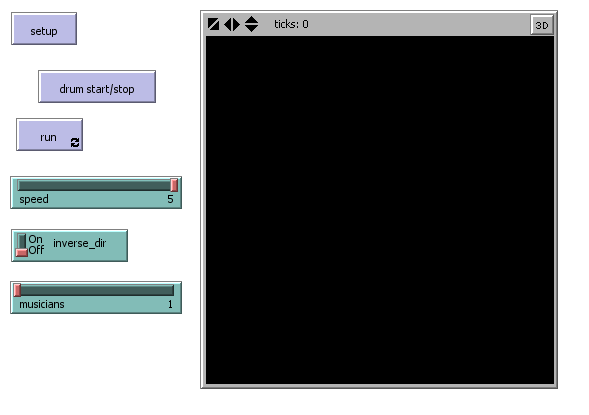
\includegraphics[scale=0.77]{fig/Trommler_interface.png}
	\caption{Trommler - Interface}
	\label{fig:Trommler.interface}
\end{figure}

Um das Programm zu starten ist es notwendig zuerst ''Setup'' und dann in 
beliebiger Reihenfolge ''drum start/stop'' und ''run'' zu dr"ucken. 
Der Knopf ''drum start/stop'' bewirkt dass der/die Trommler beginnen zu trommeln
, bzw. wieder aufh"oren zu trommeln. 

Ein Druck auf ''run'' l"asst die Trommler im Kreis marschieren, ein weiterer
Druck bewirkt, dass sie stehen bleiben. 

"Uber den Regler mit der Beschriftung speed kann die Geschwindigkeit der 
Trommler reguliert werden. Das kann auch passieren w"ahrend die Trommler schon
im Kreis marschieren.

Der Schalter ''inverse\_dir'' Entscheidet ob die Trommler alternierend gegengleich
marschieren oder nicht. Wir er auf ''On'' gesetzt, marschiert der erste Trommler
im Uhrzeigersinn, der Zweite gegen den Uhrzeigersinn und der Dritte wieder im
Uhrzeigersinn. Wird der Schalter umgelegt w"ahrend die Trommler schon marschieren
verlassen diese ihre Bahnen und beginnen von ihrem aktuellen Punkt aus wieder
in Kreisen zu marschieren, was an den Effekten der Akustik aber nichts "andert.

"Uber den Regler ''musicians'' wird die Anzahl der Trommler festgelegt. Nach 
einer "Anderung der Anzahl muss erneut auf ''setup'' gedr"uckt werden. 

\subsubsection{Funktionsweise}
Aufgrund der M"oglichkeiten, die die Erweiterung mit sich bringt ist der l"angste
Teil des Programm, die Setup-Prozedur. Sonst besteht das Programm noch aus zwei
weiteren Prozeduren: der Bewegung der Trommler und das Instruieren des Conductor.

Das Marschieren der Trommler ist simpel gehalten: Es wird lediglich berechnet,
wie weit jeder einzelne Trommler vorw"arts gehen muss, dann wird noch f"ur jeden
Trommler abh"angig davon ob sie alternierend gegengleich marschieren berechnet
wie weit er sich drehen muss. Dann wird jeder Trommler verschoben und ein
\lstinline|midi:updateposition| durchgef"uhrt. 

Das Instruieren des Conductor ist sehr einfach. Die \lstinline|drum|-Prozedur wird, von
einem Schalter am Interface aus aufgerufen. Wird noch nicht getrommelt, dh. die
Variable \lstinline|drumming| ist \lstinline|false|, wird 
"uber ein \lstinline|midi:conductor.start| der Conductor angewiesen mit dem
Musikst"uck zu beginnen und die Variable \lstinline|drumming| auf 
\lstinline|true| gesetzt. Im anderen Fall, also wenn schon getrommelt wird,
dh. die Variable \lstinline|drumming| ist \lstinline|true|, wird der Conductor
angewiesen das Musikst"uck zu beenden. Das passiert "uber den Befehl 
\lstinline|midi:conductor.stop|. Anschliesend wird noch \lstinline|drumming| auf
\lstinline|false| gesetzt. 

Das Setup des Models ist im Grunde auch einfach: F"ur drei Trommler werden die
Noten und die Instrumente definiert bzw. dem Conductor mitgeteilt (Befehle
\lstinline|midi:conductor.add.to.sheet| und \lstinline|midi:instrument|)


\subsubsection{Der Source Code im Detail}
Die Setup-Prozedur erstellt die Turtles die dann die Trommler darstellen und 
richtet das Midi-Interface sowie den Conductor ein. Es m"ussen die Instrumente
gesetzt werden, da Kanal elf und zw"olf nicht automatisch Percussion-Instrumente
verwenden. In diesem Beispiel habe ich die Variante gew"ahlt, dass der Conductor
angewiesen wird zu dirigieren, bzw. angewiesen wird mit dem Dirigieren 
aufzuh"oren. Das wird in der Prozedur \lstinline|drum| erledigt. Der Dirigent
arbeitet, nach dem er gestartet wurde im Hintergrund. (Achtung: Es sei an dieser
Stelle nochmal auf die Problematik mit Blocking-Calls hingewiesen. 
Siehe auch \ref{note-warning}). \lstinline|dosmg| f"ur Do-Something, l"asst
die Turtles wandern. 

\begin{lstlisting}[language=Logo]
extensions [midi]

globals [drumming doit]

to setup
  clear-all
  
  ;; sicher ist sicher
  midi:all.notes.off 10
  midi:all.notes.off 11
  midi:all.notes.off 12
  
  midi:conductor.clear.sheets
  midi:conductor.setplaymode.endless
  
  set drumming false
  set doit false
  
  midi:conductor.add.to.sheet 10 200 "midi:noteon 10 45 1"
  midi:conductor.add.to.sheet 10 200 "midi:noteon 10 45 0.7"
  midi:conductor.add.to.sheet 10 200 "midi:noteon 10 45 0.7"
  midi:conductor.add.to.sheet 10 200 "midi:noteon 10 45 0.7"
  ;midi:conductor.add.to.sheet 10 200 "midi:noteoff 10 45"
  
  if musicians > 1 [
  midi:conductor.add.to.sheet 11 200 "midi:noteon 11 46  1"
  midi:conductor.add.to.sheet 11 200 "midi:noteon 11 46  0.7"
  midi:conductor.add.to.sheet 11 200 "midi:noteon 11 46  0.7"
  midi:conductor.add.to.sheet 11 200 "midi:noteon 11 46  0.7"
  ]
  
  if musicians > 2 [
  midi:conductor.add.to.sheet 12 200 "midi:noteon 12 47 1"
  midi:conductor.add.to.sheet 12 200 "midi:noteon 12 47 0.7"
  midi:conductor.add.to.sheet 12 200 "midi:noteon 12 47 0.7"
  midi:conductor.add.to.sheet 12 200 "midi:noteon 12 47 0.7"
  ]
  
  ;setup the instruments
  midi:instrument 11 116
  midi:instrument 12 119
 
  ;create the turtles
  create-turtles (9 + musicians) [
    home
    facexy max-pxcor max-pycor
    rt 45
    fd who
    ifelse inverse_dir [lt (-1 ^ who) * 90 ][lt 90]
    set size 3
    ;; thicker line is easier to see
    set pen-size 3
    ;; leave a trail
    pen-down
  ]
  
  ; let the unused turtles die
  ask turtle 0 [die]
  ask turtle 1 [die]
  ask turtle 2 [die]
  ask turtle 3 [die]
  ask turtle 4 [die]
  ask turtle 5 [die]
  ask turtle 6 [die]
  ask turtle 7 [die]
  ask turtle 8 [die]
end

to dosmg
  ask turtles [
    let umf who * 2 * pi
    let turn 0.4 * speed
    
    fd 0.001 * speed * umf
    
    ifelse inverse_dir
     [lt (-1 ^ who) * turn]
     [lt turn]
    
    ; update turtle position
    midi:updateposition (who + 1)
  ]
  
  tick
end

to drum
  ifelse drumming = false[
    print "starting"
    midi:conductor.start
    set drumming true
  ]
  [
    print "stopping"
    midi:conductor.stop
    set drumming false
    set doit false
  ]
end
\end{lstlisting}





\subsubsection{Ausblick}
Ziel des Models ist es die Funktion ''midi:updateposition'' und den Conductor
auf seine ''start/stop''-F"ahigkeit zu testen. Aus diesem Grund ist das Model
sehr einfach gehalten. Ein paar Varianten um das Model zu erweitern sind:
\begin{itemize}
\item \emph{Orchester} Im aktuellen Model marschieren nur ein bis drei Trommler
im Kreis. Eine Erweiterung ist weitere Musiker mitspielen zu lassen. Das kann
"uber verschiedene Wege passieren: \begin{itemize}
\item \emph{komplett-statisch} Im Programm-Code wird festgelegt was ein
einzelner Musiker, wenn ausgew"ahlt, spielt. Das Interface wird um Switches f"ur
die einzelnen Musiker erweitert. 
\item \emph{teil-statisch} Das Interface wird erweitert, um die M"oglichkeit 
f"ur eine festgelegt Anzahl an Musikern, Noten und deren Werte einzugeben. Der
Programm-Code muss diese Werte dann in die Notenbl"atter schreiben und dem 
Conductor mitteilen. Achtung: Die Erweiterung des Interfaces um die Eingabe ist
bei weitem nicht einfach, da eine vern"unftige Struktur gefunden werden muss, 
wie die Noten und ihre Werte eingeben werden k"onnen. Auch im Programm-Code muss
dann einiges an Abfragen passieren ob einzelne Felder gesetzt sind
\item \emph{dynamisch} Die Musiker und ihre Noten werden "uber Dateien 
definiert. Das Programm wird so erweitert, dass es in einem Ordner nach Dateien
mit einem normierten Dateinamen sucht und aus diesen die Noten und ihre 
Noten-Werte ausliest. Als Format f"ur die Dateien ist ein einfaches CSV-Format
ausreichend. 
\end{itemize}
\item \emph{Marsch-Formationen} Anstatt die Trommler nur in Kreisbahnen gehen
zu lassen, kann das Model um die Funktionalit"at erweitert werden, dass sich
die Trommler auf selbst definierten Funktions-Bahnen bewegen. So kann das 
Interface um Eingabefelder erweitert werden wo f"ur jeden Trommler die Grenzen
f"ur die Funktion und die Funktion, welche abh"anig von einem Zeitparameter sein
sollte, eingegeben werden kann. Als programmiertechnische L"osung kann zB. in der
Setuproutine eine Liste mit Positions"anderungen angelegt werden, diese wird
durch schrittweise Berechnung, der einzelnen vom Benutzer eingegebenen 
Funktionen berechnet. 
\end{itemize}

\subsection{Rettungsauto}
\label{Bsp:Rettungsauto}
\subsubsection{Idee}
% Ein simuliertes Auto soll "uber den Bildschirm fahren und dabei das Martinshorn
% erklingen lassen. Es soll aber ein realistisches Modell sein, also der 
% Dopplereffekt simuliert werden.
Simulierte Rettungsautos sollen "uber den Bildschirm fahren und dabei das Martinshorn
erklingen lassen. Es soll aber ein nahezu realistisches
Model werden, was bedeutet, dass der Dopplereffekt ebenfalls simuliert
werden soll. Der Einfachheit halber gehen wir von einer kugelf"ormigen Welt aus,
die jedoch auf eine zweidimensionale Oberfl"ache abgebildet wird. Das bedeutet
nichts anderes, als das die normale NetLogo-Oberfl"ache verwendet werden kann,
die T"one sollen im zweidimensionalen Raum erscheinen und ein Auto, welches die
Welt auf der einen Seite verl"asst, soll auf der Anderen wieder hineinfahren. 
F"ur den Dopplereffekt soll davon ausgegangen werden, dass der Zuh"orer in
der Mitte, also auf der Koordinate $(0/0)$ steht. 

\subsubsection{Didaktische Aufbereitung}
Auch dieses Projekt sollte zuerst in eine Teilschritte zerlegt werden.
\begin{itemize}
\item Martins Horn
\item Dopplereffekt
\item Fahrendes Auto
\item Mehrere Autos
\end{itemize}
Wie im vorherigen Beispiel eignet sich auch hier der Schritt zuerst mit
MidiCSD die T"one zu entwickeln und dann erst mit NetLogo zu implementieren.

\begin{description}
\item[Martins Horn] Es soll ein "osterreichisches Rettungsauto modelliert werden.
Das Ziel-Instrument ist also eine Trompete. Die Lernenden sollen aber zuerst
selber raten und ausprobieren welches Instrument sich am Besten eignet. 
Ist das Instrument gefunden soll vom Ton mit dem Wert 60 aus der zweite Ton 
gefunden werden. Der Zugang kann entweder "uber das Experimentieren also das
Ausprobieren welcher Ton der Richtige ist, oder die Musik, also welches das 
richtige Intervall ist und wie dieses auf eine Midi-Tonh"ohe umgerechnet wird
gew"ahlt werden. 

\item[Dopplereffekt] Der Einfachheit halber sollte ein linearer Dopplereffekt
betrachtet werden. Sollten die Lernenden den Dopplereffekt nicht schon ausf"uhrlich
in Physik behandelt haben sollte eine Einf"uhrung in den Dopplereffekt und dessen
richtige Berechnung gegeben werden. "Uber Tabellen in Excel in denen mit der
Formel experimentiert wird, soll dann eine Formel f"ur die Berechnung entwickelt
werden. In der Beispiell"osung wird die skalierte Position des Autos mit $0.7$ 
multipliziert. Zu Beachten ist, dass in beiden F"allen mit $-1$ multipliziert wird,
da ein ansteigender Ton einen positiven Wert und ein abfallender Ton einen negativen
Wert erfordert. F"ur das verschieben des Tones gibt es den Befehl \lstinline|pitch.bend|
Dieser bekommt einen Wert zwischen $-1$ und $+1$. Pitchbending bedeutet nichts
anderes als das 'Beugen' der Tonh"ohe. 

\item[Fahrendes Auto] Das fahrende Auto ist in diesem Fall sehr einfach. Es muss
lediglich eine Turtle vorw"arts bewegt werden. Um das Model noch etwas realistischer
zu machen sollte zus"atzlich noch der UpdatePosition Befehl verwendet werden, damit
die Position auf der Ebene auch h"orbar gemacht wird. Das ganze kann "uber einen
Schieberegler der die Geschwindigkeit regeln soll und "uber den \lstinline|every|
-Befehl sehr sch"on und einfach gel"ost werden.

\item[Mehrere Autos] In diesem Schritt sollte am Besten ein Schieberegler f"ur
die Anzahl der Autos eingebaut werden. Im Setup "andert sich dann das statt
einer Turtle mehrere erstellt werden. Damit diese nicht alle parallel zu
einander fahren und auch nicht vom gleichen Punkt aus starten eignet sich
ein wiederholtes zur"uckgreifen auf Random. Im Code f"ur das Fahren "andert
sich nichts. F"ur das erstellen der Martinsh"orner ist jedoch ein kleiner
Trick erforderlich: Werden alle Autos mit den gleichen Werten f"ur die 
Notendauer versehen, klingt das nicht sehr gut. Anstatt jedes Auto bei 0 oder 1
beginnen zu lassen kann aber einfach mit \lstinline|who| begonnen werden. Das
bedeutet zwar, dass sich f"ur das zweite oder dritte Auto die T"one etwas
verschieben ist aber kaum h"orbar. Um das ganze echt Zeitversetzt zu machen,
w"aren aber einige Kunstgriffe notwendig. (Eine einfache L"osung ist aber
mit einem nicht h"orbaren Ton zu beginnen und dann in einer Schleife die T"one
f"ur das Martinshorn hinzuzuf"ugen und 'Playmode normal' auszuw"ahlen.)


\end{description}

\subsubsection{Benutzer-Oberfl"ache}

\begin{figure}[htb]
	\centering
		% width=304pt,height=225pt
		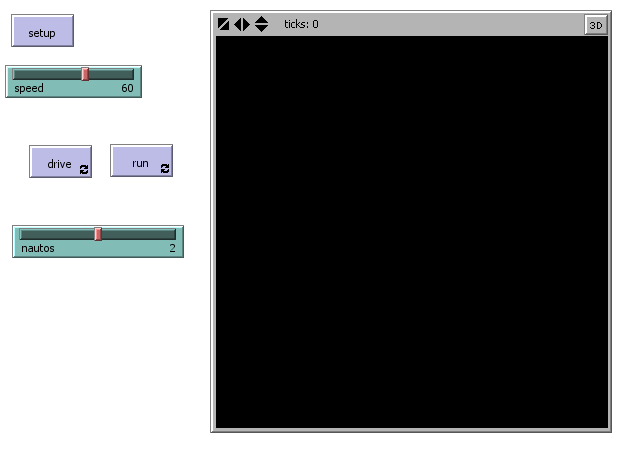
\includegraphics[scale=0.7]{fig/Rettungsauto_interface.jpg}
	\caption{Rettungsauto - Interface}
	\label{fig:Rettungsauto.interface}
\end{figure}

Die Abbildung \ref{fig:Rettungsauto.interface} zeigt die Oberfl"ache f"ur die 
Anwender des Modells. Links oben befindet sich der Knopf um das Modell zu 
initialisieren. Um die das Rettungsautofahren zulassen m"ussen die Kn"opfe
''run'' und ''drive'' gedr"uckt werden. Drive l"asst das Auto "uber die
Fl"ache fahren, w"ahrend ''run'' das Martinshorn aktiviert. 
Weiter unten befindet sich ein Regler um die Geschwindigkeit des Autos zu 
regeln. Sowie der Regler durch den sich die Anzahl der Autos festlegen l"asst. 
Diese "Anderung wird aber nur aktiv wenn erneut auf 'Setup' gedr"uckt wird. 

\subsubsection{Funktionsweise}
Das Grundprinzip des Models ist einfach: "Uber die zwei Kn"opfe werden 
unabh"angig von einander zwei Prozeduren wiederholt ausgef"uhrt. Die
Prozedur f"ur das Martinshorn enth"alt lediglich die Anweisung 
\lstinline|conductor.conduct| um das Abspielen der Midi-Befehle f"ur das 
Martinshorn zu bewirken. Die zweite Prozedur berechnet die Positions"anderung
anhand der Parameter Geschwindigkeit und vergangener Zeit. Anschlie"send 
schiebt sie die Schildkr"ote, welche das Rettungsauto repr"asentiert nach vorne
und f"uhrt ein Positions-Update f"ur die Schildkr"ote durch. 

\subsubsection{Der Source Code im Detail}
Die Setup-Prozedur erstellt das virtuelle Rettungsauto und richtet den Conductor
ein. Als Hilfsfunktion verwendet sie \lstinline|make.tatue| um die T"one f"ur
das Rettungsauto zu erzeugen. Das Beispiel verwendet in diesem Fall, als 
Unterschied zum Trommler-Beispiel die Variante den Conductor in jedem Schritt
einzeln aufzurufen und ihn dirigieren lassen. Damit kann das Auto unabh"angig von
seinem Martinshorn fahren lassen. Das Dirigieren wird in der kurzen Prozedur \lstinline|runit|
realisiert, das Fahren in \lstinline|drive|.

\begin{lstlisting}[language=Logo]
extensions [midi]

; globals [lasttick velocity lasttime]

turtles-own[channel]

to setup
  clear-all
  random-seed new-seed
  
  midi:conductor.clear.sheets
  midi:all.notes.off 1
  
  create-turtles nautos[
    set size 10
    setxy ((random 200) - 100) ((random 200) - 100)
    facexy ((random 100) - 50) ((random 50) - 25)
    set channel who + 1
    midi:updateposition channel
  ]
  
  make.tatue
    
  reset-timer
  ; set lasttime 0
end

to make.tatue
  ask turtles[
		midi:conductor.add.to.sheet channel 0 + who "midi:noteon 1 60 1"
		midi:conductor.add.to.sheet channel 250 "midi:noteoff 1 60"
		midi:conductor.add.to.sheet channel 10 "midi:noteon 1 65 1"
		midi:conductor.add.to.sheet channel 250 "midi:noteoff 1 65"
		
		midi:instrument channel 57
  ]
  
  midi:conductor.setplaymode.endless
end

to runit
  midi:conductor.conduct
end

to drive
  every 0.25 [
  ask turtles [
    fd speed * 0.1
    
    every 1 [ midi:updateposition channel]
    
    if xcor < 0 [
      midi:pitch.bend channel ( 0.7 / min-pxcor * xcor * -1 )
    ]
    if xcor = 0 [ midi:pitch.bend channel 0]
    if xcor > 0 [
      midi:pitch.bend channel ( 0.7 / max-pxcor * xcor * -1 )
    ]
  ]
  
  ]
  
  tick  
end
\end{lstlisting}


\subsubsection{Ausblick}
Das Modell zeigt zur Zeit nur elementare F"ahigkeiten der Midi-Extension, kann
aber nat"urlich beliebig erweitert werden. 
\begin{itemize}
\item \emph{Mehr Fahrzeuge: }
Das Modell kann nat"urlich um weitere Autos erweitert werden. So ist es 
m"oglich "uber den Dirigenten Notenbl"atter f"ur die verschiedenen Fahrzeuge
anzulegen. So kann das Model sehr einfach um Feuerwehr, Polizei, oder anderes
erweitert werden. Soll sich auch die Art der Fortbewegung "andern muss die 
drive-Prozedur ver"andert werden. 
\item \emph{Hindernisse: }
Im aktuellen Model fahren die Autos ungehindert durch die Welt. Durch einfache
"Anderungen am Modell k"onnten breeds als Hindernisse deklariert werden. F"ahrt
ein Auto auf eines von diesen auf, soll eine Aktion ausgef"uhrt werden (zB das
Auto soll wenden, also eine 180 Grad Drehung machen)
\item \emph{Fahrtverl"aufe: } 
In der aktuellen Implementierung kann lediglich der Startpunkt des Autos gesetzt
werden, nicht jedoch der Verlauf der Fahrt. Ein m"ogliche Erweiterung ist, dass
der Benutzer aus mehreren Funktionen ausw"ahlen oder diese auch selber eingeben 
kann, welche den Verlauf der Fahrt berechnen.
\item \emph{Genauerer Dopplereffekt: }
Der Dopplereffekt wird im vorliegenden Modell nur approximiert. Durch Literatur-Recherche und 
geringf"ugige "Anderungen am Code, kann sehr einfach eine bessere Ann"aherung
erreicht werden. 
\end{itemize}


% \section{Source Code}
\lstset{tabsize=2}
\lstset{captionpos=b} %caption pos on bottom of the code
\lstset{breaklines=true}
\lstset{linewidth=\textwidth}
\lstset{basicstyle=\small\textit\ttfamily}

\subsection{ Cmd.java }
\lstinputlisting[language=Java]{ ../midi/src/at/univie/csd/Cmd.java }
\subsection{ AllNotesOff.java }
\lstinputlisting[language=Java]{ ../midi/src/at/univie/csd/command/AllNotesOff.java }
\subsection{ ChannelPressure.java }
\lstinputlisting[language=Java]{ ../midi/src/at/univie/csd/command/ChannelPressure.java }
\subsection{ Chorus.java }
\lstinputlisting[language=Java]{ ../midi/src/at/univie/csd/command/Chorus.java }
\subsection{ ConductorAddToSheet.java }
\lstinputlisting[language=Java]{ ../midi/src/at/univie/csd/command/ConductorAddToSheet.java }
\subsection{ ConductorAddToSheetWT.java }
\lstinputlisting[language=Java]{ ../midi/src/at/univie/csd/command/ConductorAddToSheetWT.java }
\subsection{ ConductorClearSheets.java }
\lstinputlisting[language=Java]{ ../midi/src/at/univie/csd/command/ConductorClearSheets.java }
\subsection{ ConductorConduct.java }
\lstinputlisting[language=Java]{ ../midi/src/at/univie/csd/command/ConductorConduct.java }
\subsection{ ConductorPlaymodeEndless.java }
\lstinputlisting[language=Java]{ ../midi/src/at/univie/csd/command/ConductorPlaymodeEndless.java }
\subsection{ ConductorPlaymodeNormal.java }
\lstinputlisting[language=Java]{ ../midi/src/at/univie/csd/command/ConductorPlaymodeNormal.java }
\subsection{ ConductorReset.java }
\lstinputlisting[language=Java]{ ../midi/src/at/univie/csd/command/ConductorReset.java }
\subsection{ ConductorStart.java }
\lstinputlisting[language=Java]{ ../midi/src/at/univie/csd/command/ConductorStart.java }
\subsection{ ConductorStop.java }
\lstinputlisting[language=Java]{ ../midi/src/at/univie/csd/command/ConductorStop.java }
\subsection{ Controller.java }
\lstinputlisting[language=Java]{ ../midi/src/at/univie/csd/command/Controller.java }
\subsection{ Expression.java }
\lstinputlisting[language=Java]{ ../midi/src/at/univie/csd/command/Expression.java }
\subsection{ Instrument.java }
\lstinputlisting[language=Java]{ ../midi/src/at/univie/csd/command/Instrument.java }
\subsection{ KeyPressure.java }
\lstinputlisting[language=Java]{ ../midi/src/at/univie/csd/command/KeyPressure.java }
\subsection{ MastertuneCoarse.java }
\lstinputlisting[language=Java]{ ../midi/src/at/univie/csd/command/MastertuneCoarse.java }
\subsection{ MastertuneFine.java }
\lstinputlisting[language=Java]{ ../midi/src/at/univie/csd/command/MastertuneFine.java }
\subsection{ Modulation.java }
\lstinputlisting[language=Java]{ ../midi/src/at/univie/csd/command/Modulation.java }
\subsection{ Note.java }
\lstinputlisting[language=Java]{ ../midi/src/at/univie/csd/command/Note.java }
\subsection{ NoteOff.java }
\lstinputlisting[language=Java]{ ../midi/src/at/univie/csd/command/NoteOff.java }
\subsection{ NoteOn.java }
\lstinputlisting[language=Java]{ ../midi/src/at/univie/csd/command/NoteOn.java }
\subsection{ Nrpn.java }
\lstinputlisting[language=Java]{ ../midi/src/at/univie/csd/command/Nrpn.java }
\subsection{ Pan.java }
\lstinputlisting[language=Java]{ ../midi/src/at/univie/csd/command/Pan.java }
\subsection{ Panic.java }
\lstinputlisting[language=Java]{ ../midi/src/at/univie/csd/command/Panic.java }
\subsection{ PitchBend.java }
\lstinputlisting[language=Java]{ ../midi/src/at/univie/csd/command/PitchBend.java }
\subsection{ PitchSens.java }
\lstinputlisting[language=Java]{ ../midi/src/at/univie/csd/command/PitchSens.java }
\subsection{ Portamento.java }
\lstinputlisting[language=Java]{ ../midi/src/at/univie/csd/command/Portamento.java }
\subsection{ PortamentoFrom.java }
\lstinputlisting[language=Java]{ ../midi/src/at/univie/csd/command/PortamentoFrom.java }
\subsection{ PortamentoTime.java }
\lstinputlisting[language=Java]{ ../midi/src/at/univie/csd/command/PortamentoTime.java }
\subsection{ ResetControllers.java }
\lstinputlisting[language=Java]{ ../midi/src/at/univie/csd/command/ResetControllers.java }
\subsection{ Reverb.java }
\lstinputlisting[language=Java]{ ../midi/src/at/univie/csd/command/Reverb.java }
\subsection{ Rpn.java }
\lstinputlisting[language=Java]{ ../midi/src/at/univie/csd/command/Rpn.java }
\subsection{ Sustain.java }
\lstinputlisting[language=Java]{ ../midi/src/at/univie/csd/command/Sustain.java }
\subsection{ UpdatePosition.java }
\lstinputlisting[language=Java]{ ../midi/src/at/univie/csd/command/UpdatePosition.java }
\subsection{ Volume.java }
\lstinputlisting[language=Java]{ ../midi/src/at/univie/csd/command/Volume.java }
\subsection{ Conversion.java }
\lstinputlisting[language=Java]{ ../midi/src/at/univie/csd/Conversion.java }
\subsection{ Conductor.java }
\lstinputlisting[language=Java]{ ../midi/src/at/univie/csd/midi/Conductor.java }
\subsection{ ConductorThread.java }
\lstinputlisting[language=Java]{ ../midi/src/at/univie/csd/midi/ConductorThread.java }
\subsection{ Sheet.java }
\lstinputlisting[language=Java]{ ../midi/src/at/univie/csd/midi/Sheet.java }
\subsection{ TimedEvent.java }
\lstinputlisting[language=Java]{ ../midi/src/at/univie/csd/midi/TimedEvent.java }
\subsection{ MidiCommand.java }
\lstinputlisting[language=Java]{ ../midi/src/at/univie/csd/MidiCommand.java }
\subsection{ MidiContext.java }
\lstinputlisting[language=Java]{ ../midi/src/at/univie/csd/MidiContext.java }
\subsection{ MidiManager.java }
\lstinputlisting[language=Java]{ ../midi/src/at/univie/csd/MidiManager.java }
\subsection{ TwoByte.java }
\lstinputlisting[language=Java]{ ../midi/src/at/univie/csd/TwoByte.java }



\addcontentsline{toc}{section}{Literaturverzeichnis}
\bibliographystyle{amsplain} %take natbib if you need refernces by Author&year
\bibliography{lit}

\end{document}

